Waves emminate from a source

These waves reflect off the antenna in such a way to be directed towards a target

The problem is how to calculate the scattering pattern off an antenna

Setting reflection at the antenna surface ($S_A$)

$$\left.\psi \right|_{S_A} = 0$$

\begin{center}
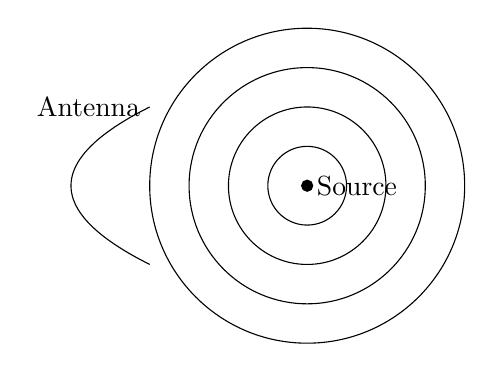
\begin{tikzpicture}
    \filldraw [black] (3,0) circle (2pt) node [anchor=west] {Source};
    \draw [smooth,domain=-1:1,variable=\y] plot({\y*\y},{\y})
    node [anchor=east] {Antenna};
    \draw (3.5,0) arc (0:360:0.5);
    \draw (4,0) arc (0:360:1);
    \draw (4.5,0) arc (0:360:1.5);
    \draw (5,0) arc (0:360:2);
\end{tikzpicture}
\end{center}